%
\documentclass[runningheads]{llncs}
%
\usepackage{graphicx}
\usepackage{comment}
\usepackage{xcolor}
% Used for displaying a sample figure. If possible, figure files should
% be included in EPS format.
%
% If you use the hyperref package, please uncomment the following line
% to display URLs in blue roman font according to Springer's eBook style:
% \renewcommand\UrlFont{\color{blue}\rmfamily}

\begin{document}
%
\title{Membrane-localized Keratin-14 Promotes Invasion\thanks{Supported by organization x.}}
%
%\titlerunning{Abbreviated paper title}
% If the paper title is too long for the running head, you can set
% an abbreviated paper title here
%
\author{First Author \inst{1}\orcidID{0000-1111-2222-3333} \and
Second Author\inst{2,3}\orcidID{1111-2222-3333-4444} \and
Third Author\inst{3}\orcidID{2222--3333-4444-5555}}
%
\authorrunning{F. Author et al.}
% First names are abbreviated in the running head.
% If there are more than two authors, 'et al.' is used.
%
\institute{Johns Hopkins University
\url{http://www} \and
Other\\
\email{\{bla,blu\}@jhu.edu}}
%
\maketitle              % typeset the header of the contribution
%
\begin{abstract}
Metastasis is the main predictor of outcome for patients with cancer, yet the molecular mechanism driving invasive phenotypes is not well understood. Keratin 14 (K14) is a known molecular biomarker that is correlated with poor outcomes in breast cancer patients. In this study, we apply our automated computer model that quantifies the invasive potential of tumors to characterize K14 expression as it relates to invasion. We test the hypothesis that K14 is directly correlated to invasion versus the alternative hypothesis that size is the main predictor. We used two different transgenic mice (PyMT and C3(1)-Tag) as our breast cancer tumor models. Organoids were generated from these mice, and each organoid had a corresponding differential interference contrast image, K14 image, and an invasive potential score generated using our automated system. The parameters assessed include the following: entire K14 expression, peripheral K14 expression (edges of the organoid), central K14 expression (center of the organoid), and organoid size. Peripheral K14 expression showed the strongest correlation with invasion scores for both types of transgenic mice. The results suggest that K14 expression in cells located in the periphery may be an important marker of invasion.

\keywords{Metastasis \and Tumor Invasion \and Keratin 14 \and Spectral Analysis \and ...}
\end{abstract}
%
%
%
\section{Introduction}

Alternative title: Morphological features of organoid invasion are correlated to membrane-localized Keratin-14 expression

\textcolor{blue}{
\begin{itemize}
    \item Biology intro (what is our audience). The two different mice models.
    \item How K14 expression is related to metastasis.
    \item The use of image analysis for feature extraction, lit review.
    \item Why spectral score is a good measure for invasion potential.
    \item Paper outline
\end{itemize}
}

Metastasis stats.

What are organoids.

Quantitative phenotypes.


Hypothesis: a) K14 expression is correlated with organoid invasion.\\
b) organoid size is correlated with invasion score.

Research questions:


\section {Methods}

Fig. 0: Make figure showing the 'pipeline'.

\textcolor{blue}{
\begin{itemize}
    \item Experimental protocol. Ask Veena to write this part.\\ 
        100-300 organoids from 4 mice.
    \item Image acquisition and organoid periphery. Veena.\\
        Use ImageJ to mark the periphery of the organoids from DCI microscop images.
    \item Image segmentation. Andrei to write about convolution kernel.
    \item Spectral score. Reference Joel's paper. Disclose scripts?
\end{itemize}
}

\subsection{Dataset}

 A total of 4 PyMT and 4 C31T mice were used to generate a total of \{\} organoids, which were then cultured in collagen I gels for 5 days. At day 5, they were imaged, an average of 16 per sample. Differential interference contrast (DIC) microscopy yielded 1040$\times$1388 pixel images. Microscope optics defined a resolution of 0.51190476 $\mu$m per pixel, corresponding to a 532.4$\times$710.5 $\mu$m field of view. Images were manually tracked in {\sc ImageJ} \cite{Schneider:2012ui} to define the organoid boundaries as pairs of points $\{x_v,y_v\}$ for $v \in [0,V-1]$. The total number of points $V$ depended on the manual tracking, and the spacing between adjacent points was similarly variable.

\subsection{Spectral Analysis}

\subsubsection{}

\section{Results}

Start adding figures here.\\
Q: Are we keeping the large vs. small organoids?
Q: should this be split into PyMT section and C31Tag section?

Fig. 1: show each step in the pipeline from DCI to spectral score for 2 organoids (one with low spectral score and one with high spectral score).

Fig. 2: show figures for the convolution kernel used to get peripheral K14 expression.

Fig. 3: Correlation plots PyMT

Fig. 4: Correlation plots C31Tag

Table 1: Summary statistics

\section{Discussion}

Future directions: Test our method on Patient derived organoids, PDOs.\\
Does organoid invasion score correlate with patient outcome?

\section{Conclusion}




%%%%%%%%%%%%%%%%%%%%%%%%%%%%%%%%%%%%%%%
\begin{comment}
\begin{table}
\caption{Table captions should be placed above the
tables.}\label{tab1}
\begin{tabular}{|l|l|l|}
\hline
Heading level &  Example & Font size and style\\
\hline
Title (centered) &  {\Large\bfseries Lecture Notes} & 14 point, bold\\
1st-level heading &  {\large\bfseries 1 Introduction} & 12 point, bold\\
2nd-level heading & {\bfseries 2.1 Printing Area} & 10 point, bold\\
3rd-level heading & {\bfseries Run-in Heading in Bold.} Text follows & 10 point, bold\\
4th-level heading & {\itshape Lowest Level Heading.} Text follows & 10 point, italic\\
\hline
\end{tabular}
\end{table}


\noindent Displayed equations are centered and set on a separate
line.
\begin{equation}
x + y = z
\end{equation}
Please try to avoid rasterized images for line-art diagrams and
schemas. Whenever possible, use vector graphics instead (see
Fig.~\ref{fig1}).

\begin{figure}
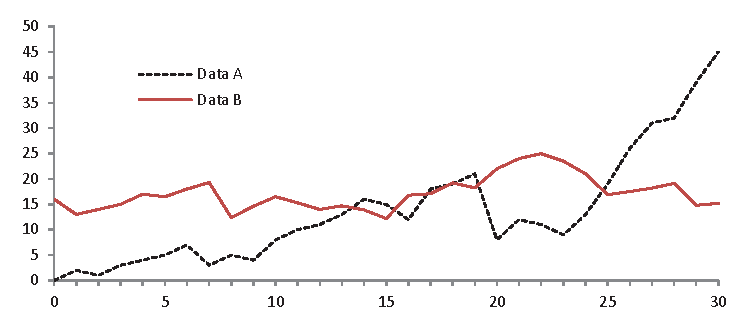
\includegraphics[width=\textwidth]{fig1.eps}
\caption{A figure caption is always placed below the illustration.
Please note that short captions are centered, while long ones are
justified by the macro package automatically.} \label{fig1}
\end{figure}

\begin{theorem}
This is a sample theorem. The run-in heading is set in bold, while
the following text appears in italics. Definitions, lemmas,
propositions, and corollaries are styled the same way.
\end{theorem}
%
% the environments 'definition', 'lemma', 'proposition', 'corollary',
% 'remark', and 'example' are defined in the LLNCS documentclass as well.
%
\begin{proof}
Proofs, examples, and remarks have the initial word in italics,
while the following text appears in normal font.
\end{proof}
For citations of references, we prefer the use of square brackets
and consecutive numbers. Citations using labels or the author/year
convention are also acceptable. The following bibliography provides
a sample reference list with entries for journal
articles~\cite{ref_article1}, an LNCS chapter~\cite{ref_lncs1}, a
book~\cite{ref_book1}, proceedings without editors~\cite{ref_proc1},
and a homepage~\cite{ref_url1}. Multiple citations are grouped
\cite{ref_article1,ref_lncs1,ref_book1},
\cite{ref_article1,ref_book1,ref_proc1,ref_url1}.
%
% ---- Bibliography ----
%
% BibTeX users should specify bibliography style 'splncs04'.
% References will then be sorted and formatted in the correct style.
%
% \bibliographystyle{splncs04}
% \bibliography{mybibliography}
%

\end{comment}

\begin{thebibliography}{8}

\bibitem{Schneider:2012ui}
Schneider CA, Rasband WS, Eliceiri KW.
\newblock {NIH Image to ImageJ: 25 years of image analysis.}
\newblock Nature methods. 2012;9(7):671--675.

\end{thebibliography}



\end{document}
